\documentclass[]{article}

% Imported Packages
%------------------------------------------------------------------------------
\usepackage{amssymb}
\usepackage{amstext}
\usepackage{amsthm}
\usepackage{amsmath}
\usepackage{enumerate}
\usepackage{fancyhdr}
\usepackage[margin=1in]{geometry}
\usepackage{graphicx}
\usepackage{extarrows}
\usepackage{setspace}
%------------------------------------------------------------------------------

% Header and Footer
%------------------------------------------------------------------------------
\pagestyle{plain}  
\renewcommand\headrulewidth{0.4pt}                                      
\renewcommand\footrulewidth{0.4pt}                                    
%------------------------------------------------------------------------------

% Title Details
%------------------------------------------------------------------------------
\title{SE 3A04: Software Design II -- Large System Design}
\author{Team 11}
\date{}  
                             
%------------------------------------------------------------------------------

% Document
%------------------------------------------------------------------------------

\begin{document}

\maketitle
\begin{center}
\hrule
	\vspace{0.2in}
\huge AudioVal.ly
	\vspace{0.05in}
\hrule
	\vspace{0.2in}
\huge  Deliverable 2 - High-Level Architectural Design
	\vspace{0.2in}

\large March 9, 2018
\\
	\vspace{1in}
			\large Team 11
\end{center}
\begin{minipage}[c]{\linewidth}
%\fontsize{14pt}{25pt}\selectfont
			\large
			\centering
			\begin{tabular}{l c c}
				Baltej Toor & 1413818 & toorbs \\
				Brandon Roberts & 400018117 & roberb1 \\
				Corey Szeto & 400025728 & szetoc \\
				Jiahong Dong & 1452923 & dongjh \\
				Puru Jetly & 1417837 & jetlyp \\
			\end{tabular}
\end{minipage}	
\newpage

\tableofcontents
\newpage
\section{Introduction}
\label{sec:introduction}
% Begin Section

This section outlines the purpose and provides a system description of the AudioVal.ly project; along with an overview of the contents and organization of this high-level architectural design document.
 


\subsection{Purpose}
\label{sub:purpose}
% Begin SubSection
The purpose of this document to define the use cases, layout the Analysis Class Diagram, describe the Architectural Design, and finally document the class responsibilities through collaboration cards. This document builds on top of and extends the Software Requirements Specification document in that this document describes the way in which the system will interact with the outside world and how the subsystems will be architecturally and logically arranged. \\
The target audience for this document are the stakeholders (Dr. Ridha Khedri, Spencer Deevy and Andrew Le Clair), and any current or future architects, designers and developers of this project.
% End SubSection

\subsection{System Description}
\label{sub:system_description}
% Begin SubSection
The AudioVal.ly application is intended to be a means to identify different genres of music.
The primary interface between the user and the software system is through a device running the Android operating system. This document defines the way in which the users will be expected to interact with the system and how the application will be decomposed into smaller subsystems to reduce the complexity and improve the maintainability, flexibility of this system.

Specifically, the users of this system (application) are expected to perform a set of events that will prompt the system to react. The decomposition will then show how the subsystems will communicate among one another in order to efficiently distribute the work and perform the required actions in response to the user's actions.

% End SubSection

\subsection{Overview}
\label{sub:overview}
% Begin SubSection
The remainder of the document is organized into 4 sections: Use Case Diagram -- how the users and system will interact, Analysis Class Diagram -- the subsystems that compose this entire application, Architectural Design -- the layout of the subsystems into a well-understood software architecture, and Class responsibility collaboration Cards -- description of the interactions between the subsystems. Each section uses an appropriate notation and diagrams
to document the design decision and describe the details of the high-level design of this system.

% End SubSection

% End Section
\newpage
\section{Use Case Diagram}
\label{sec:use_case_diagram}
% Begin Section
\begin{center}
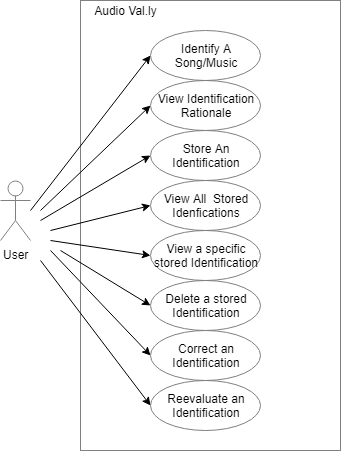
\includegraphics[scale=0.5]{uc}
\end{center}
% End Section

\newpage
\section{Analysis Class Diagram}
\label{sec:analysis_class_diagram}
% Begin Section
\begin{center}
BE1.4 The user wants to check a previously identified music genre.
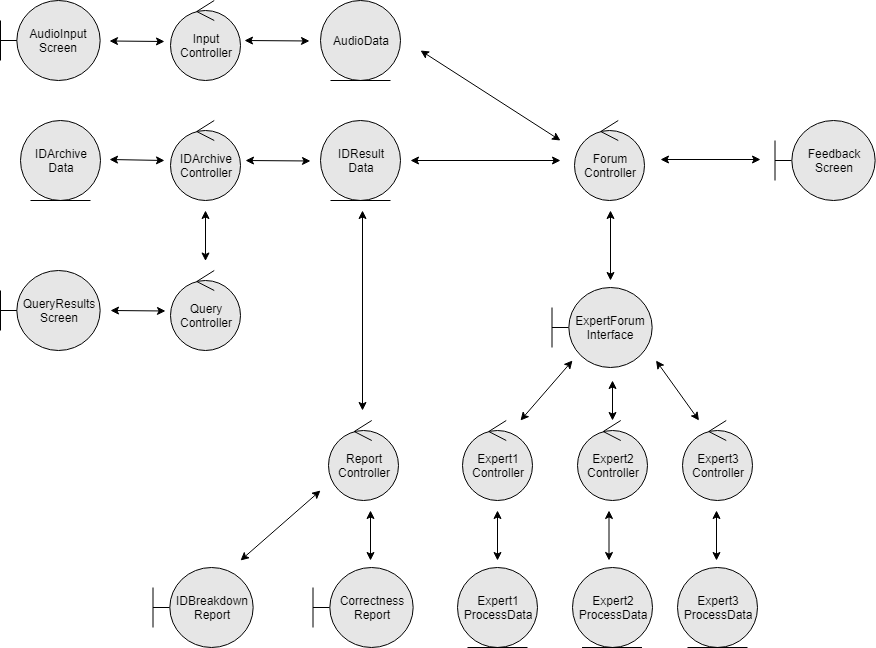
\includegraphics[scale=0.5]{analysisclass}
\end{center}
% End Section

\newpage
\section{Architectural Design}
\label{sec:architectural_design}
% Begin Section
This section should provide an overview of the overall architectural design of your application. You overall architecture should show the division of the system into subsystems with high cohesion and low coupling.

\subsection{System Architecture}
\label{sub:system_architecture}
% Begin SubSection
For our system, we use the blackboard architecture. Generally, our system consists of five major subsystems which are user interface, input, experts, forum and datastore and beside these five major subsystems, additional subsystems are reporting, history and querying. blackboard architecture is used when there are no deterministic solution strategies are known and several specialized subsystems will assemble their knowledge to build a possibly partial or approximate solution. In our case, we do not have any ideas about the genre of the music that we are identifying, and three experts only have their specialized knowledge, they can only provide a piece of information according to their limited knowledge and the forum combines the information together to a final solution. Experts work independently, they do not need to know the existence of others, therefore we use blackboard architecture. Since we use blackboard architecture, the blackboard is the forum, knowledge sources are experts and finally the control is the datastore.
% End SubSection

\subsection{Subsystems}
\label{sub:subsystems}
% Begin SubSection
The purpose of our user interface is give users the ability to operate the system, it interacts with the input subsystem and enables the user to record raw audio piece, the input subsystem records raw audio piece and then send the audio input to the expert. The expert subsystem consists of three individual experts which have their unique knowledge, expert analyzes the audio input from the input and send their partial solution to the forum. The forum collects all the partial solutions from previous expert and then gives an overall final solution. If there are conflicts, then the forum with interacts with the querying subsystem to resolve the conflicts and then return the solution back to itself. The forum also interacts with the user interface via a reporting subsystem, generate a report of the overall solution. The forum also stores the final solution to a history subsystem and this history subsystem interacts with the user interface to provides the user with previously identified solutions.
% End SubSection

% End Section

\newpage	
\section{Class Responsibility Collaboration (CRC) Cards}
\label{sec:class_responsibility_collaboration_crc_cards}
% Begin Section

	
	\begin{table}[ht]
		\centering
		\begin{tabular}{|p{5cm}|p{5cm}|}
		\hline 
		 \multicolumn{2}{|l|}{\textbf{Class Name: AudioInputScreen}} \\
		\hline
		\textbf{Responsibility:} & \textbf{Collaborators:} \\
		\hline
		Allow user to input audio for identification &  \\
		\hline
		Receive audio information from the device microphone &  \\
		\hline
		Display input validation errors &  \\
		\hline
		Receive request to take audio input & InputController \\
		\hline
		\end{tabular}
	\end{table}
	
	\begin{table}[ht]
		\centering
		\begin{tabular}{|p{5cm}|p{5cm}|}
		\hline 
		 \multicolumn{2}{|l|}{\textbf{Class Name: InputController}} \\
		\hline
		\textbf{Responsibility:} & \textbf{Collaborators:} \\
		\hline
		Store valid audio information in audio data storage & AudioInputScreen, AudioData \\
		\hline
		Validate audio input &  \\
		\hline
		Request audio input & AudioInputScreen \\
		\hline
		\end{tabular}
	\end{table}
	
	\begin{table}[ht]
		\centering
		\begin{tabular}{|p{5cm}|p{5cm}|}
		\hline 
		 \multicolumn{2}{|l|}{\textbf{Class Name: AudioData}} \\
		\hline
		\textbf{Responsibility:} & \textbf{Collaborators:} \\
		\hline
		Represent validated audio information inputted by user & \\
		\hline
		\end{tabular}
	\end{table}
	
\newpage
	\begin{table}[ht]
		\centering
		\begin{tabular}{|p{5cm}|p{5cm}|}
		\hline 
		 \multicolumn{2}{|l|}{\textbf{Class Name: ForumController}} \\
		\hline
		\textbf{Responsibility:} & \textbf{Collaborators:} \\
		\hline
		Distribute stored audio data to Expert(s) for processing & AudioData, ExpertForumInterface \\
		\hline
		Receive Expert(s) identification results & ExpertForumInterface \\
		\hline
		Resolve conflict between conflicting Expert identifications & \\
		\hline
		Store identification result report to identification storage & IDResultData \\
		\hline
		Send feedback/update information to Expert(s) & ExpertForumInterface, FeedbackScreen \\
		\hline
		Send overall identification result to FeedbackScreen & FeedbackScreen \\
		\hline
		Prompt FeedbackScreen to display result & FeedbackScreen \\
		\hline
		Receive correctness data/result correction for the identification & FeedbackScreen \\
		\hline
		Store correction data to identification storage & IDResultData \\
		\hline
		\end{tabular}
	\end{table}
	
	\begin{table}[ht]
		\centering
		\begin{tabular}{|p{5cm}|p{5cm}|}
		\hline 
		 \multicolumn{2}{|l|}{\textbf{Class Name: FeedbackScreen}} \\
		\hline
		\textbf{Responsibility:} & \textbf{Collaborators:} \\
		\hline
		Receive identification result & ForumController \\
		\hline
		Display identification result & xd \\
		\hline
		Allow user to provide correctness feedback on result & xd \\
		\hline
		Receive correctness feedback from user & xd \\
		\hline
		Compare user correction to determined identification result & xd \\
		\hline
		Send individual Expert correctness data/result correction for the identification to Forum to store & ForumController \\
		\hline
		\end{tabular}
	\end{table}
	
\newpage
	\begin{table}[ht]
		\centering
		\begin{tabular}{|p{5cm}|p{5cm}|}
		\hline 
		 \multicolumn{2}{|l|}{\textbf{Class Name: ExpertForumInterface}} \\
		\hline
		\textbf{Responsibility:} & \textbf{Collaborators:} \\
		\hline
		Pass initial audio data from Forum and Expert(s) & ForumController, Expert1Controller, Expert2Controller, Expert3Controller \\
		\hline
		Pass identification result(s) from Expert(s) to Forum &  \\
		\hline
		Transfer updates between Forum and Expert(s) &  \\
		\hline
		\end{tabular}
	\end{table}
	
	\begin{table}[ht]
		\centering
		\begin{tabular}{|p{5cm}|p{5cm}|}
		\hline 
		 \multicolumn{2}{|l|}{\textbf{Class Name: Expert1Controller}} \\
		\hline
		\textbf{Responsibility:} & \textbf{Collaborators:} \\
		\hline
		Receive audio data & ExpertForumInterface \\
		\hline
		Process audio data based on specified computation criteria &  \\
		\hline
		Store information in ProcessData & Expert1ProcessData \\
		\hline
		Determine identification result based on processing &  \\
		\hline
		Send identification result to Forum & ExpertForumInterface \\
		\hline
		Receive information (updates) from Forum & ExpertForumInterface \\
		\hline
		Utilize ProcessData for identification & Expert1ProcessData \\
		\hline
		\end{tabular}
	\end{table}
	
\newpage
	\begin{table}[ht]
		\centering
		\begin{tabular}{|p{5cm}|p{5cm}|}
		\hline 
		 \multicolumn{2}{|l|}{\textbf{Class Name: Expert2Controller}} \\
		\hline
		\textbf{Responsibility:} & \textbf{Collaborators:} \\
		\hline
		Receive audio data & ExpertForumInterface \\
		\hline
		Process audio data based on specified computation criteria &  \\
		\hline
		Store information in ProcessData & Expert2ProcessData \\
		\hline
		Determine identification result based on processing &  \\
		\hline
		Send identification result to Forum & ExpertForumInterface \\
		\hline
		Receive information (updates) from Forum & ExpertForumInterface \\
		\hline
		Utilize ProcessData for identification & Expert2ProcessData \\
		\hline
		\end{tabular}
	\end{table}

	\begin{table}[ht]
		\centering
		\begin{tabular}{|p{5cm}|p{5cm}|}
		\hline 
		 \multicolumn{2}{|l|}{\textbf{Class Name: Expert3Controller}} \\
		\hline
		\textbf{Responsibility:} & \textbf{Collaborators:} \\
		\hline
		Receive audio data & ExpertForumInterface \\
		\hline
		Process audio data based on specified computation criteria &  \\
		\hline
		Store information in ProcessData & Expert3ProcessData \\
		\hline
		Determine identification result based on processing &  \\
		\hline
		Send identification result to Forum & ExpertForumInterface \\
		\hline
		Receive information (updates) from Forum & ExpertForumInterface \\
		\hline
		Utilize ProcessData for identification & Expert3ProcessData \\
		\hline
		\end{tabular}
	\end{table}	
	
	\begin{table}[ht]
		\centering
		\begin{tabular}{|p{5cm}|p{5cm}|}
		\hline 
		 \multicolumn{2}{|l|}{\textbf{Class Name: Expert1ProcessData}} \\
		\hline
		\textbf{Responsibility:} & \textbf{Collaborators:} \\
		\hline
		Represent Expert 1 processing information/data &  \\
		\hline
		Allow updates from Expert 1 & Expert1Controller \\
		\hline
		Represent identification result for the Expert 1 &  \\
		\hline
		\end{tabular}
	\end{table}
	
\newpage
	\begin{table}[ht]
		\centering
		\begin{tabular}{|p{5cm}|p{5cm}|}
		\hline 
		 \multicolumn{2}{|l|}{\textbf{Class Name: Expert2ProcessData}} \\
		\hline
		\textbf{Responsibility:} & \textbf{Collaborators:} \\
		\hline
		Represent Expert 2 processing information/data &  \\
		\hline
		Allow updates from Expert 2 & Expert2Controller \\
		\hline
		Represent identification result for the Expert 2 &  \\
		\hline
		\end{tabular}
	\end{table}
	
	\begin{table}[ht]
		\centering
		\begin{tabular}{|p{5cm}|p{5cm}|}
		\hline 
		 \multicolumn{2}{|l|}{\textbf{Class Name: Expert3ProcessData}} \\
		\hline
		\textbf{Responsibility:} & \textbf{Collaborators:} \\
		\hline
		Represent Expert 3 processing information/data &  \\
		\hline
		Allow updates from Expert 3 & Expert3Controller \\
		\hline
		Represent identification result for the Expert 3 &  \\
		\hline
		\end{tabular}
	\end{table}
	
	\begin{table}[ht]
		\centering
		\begin{tabular}{|p{5cm}|p{5cm}|}
		\hline 
		 \multicolumn{2}{|l|}{\textbf{Class Name: IDResultData}} \\
		\hline
		\textbf{Responsibility:} & \textbf{Collaborators:} \\
		\hline
		Represent identification result data &  \\
		\hline
		Allow updates by Forum &  \\
		\hline
		\end{tabular}
	\end{table}
	
\newpage
	\begin{table}[ht]
		\centering
		\begin{tabular}{|p{5cm}|p{5cm}|}
		\hline 
		 \multicolumn{2}{|l|}{\textbf{Class Name: IDArchiveController}} \\
		\hline
		\textbf{Responsibility:} & \textbf{Collaborators:} \\
		\hline
		Retrieve identification result information & IDResultData \\
		\hline
		Archive identification result information & IDArchiveData \\
		\hline
		Receive query on identification archive & QueryController \\
		\hline
		Perform query on identification archive &  \\
		\hline
		Return query result & QueryController \\
		\hline
		Receive deletion request of archive data & QueryController \\
		\hline
		Delete specified archive data &  \\
		\hline
		\end{tabular}
	\end{table}
	
	\begin{table}[ht]
		\centering
		\begin{tabular}{|p{5cm}|p{5cm}|}
		\hline 
		 \multicolumn{2}{|l|}{\textbf{Class Name: IDArchiveData}} \\
		\hline
		\textbf{Responsibility:} & \textbf{Collaborators:} \\
		\hline
		Represent historical identification result(s) data &  \\
		\hline
		\end{tabular}
	\end{table}
	
	\begin{table}[ht]
		\centering
		\begin{tabular}{|p{5cm}|p{5cm}|}
		\hline 
		 \multicolumn{2}{|l|}{\textbf{Class Name: QueryController}} \\
		\hline
		\textbf{Responsibility:} & \textbf{Collaborators:} \\
		\hline
		Request query on archived identification data & IDArchiveController \\
		\hline
		Receive query result & IDArchiveController \\
		\hline
		Prompt ResultsScreen to display query result & QueryResultsScreen \\
		\hline
		Request archive data deletion & IDArchiveController \\
		\hline
		Display deletion confirmation &  \\
		\hline
		\end{tabular}
	\end{table}
	
\newpage
	\begin{table}[ht]
		\centering
		\begin{tabular}{|p{5cm}|p{5cm}|}
		\hline 
		 \multicolumn{2}{|l|}{\textbf{Class Name: QueryResultsScreen}} \\
		\hline
		\textbf{Responsibility:} & \textbf{Collaborators:} \\
		\hline
		Receive query result on identification archive & QueryController \\
		\hline
		Display query result to user &  \\
		\hline
		Display archived identification data &  \\
		\hline
		Respond to Delete result record from archive & QueryController \\
		\hline
		\end{tabular}
	\end{table}
	
	\begin{table}[ht]
		\centering
		\begin{tabular}{|p{5cm}|p{5cm}|}
		\hline 
		 \multicolumn{2}{|l|}{\textbf{Class Name: ReportController}} \\
		\hline
		\textbf{Responsibility:} & \textbf{Collaborators:} \\
		\hline
		Receive information on recent identification result and processing & IDResultData \\
		\hline
		Generate report based on specified criteria & xd \\
		\hline
		Prompt corresponding screen to display report & IDBreakdownReport, CorrectnessReport \\
		\hline
		\end{tabular}
	\end{table}
	
	\begin{table}[ht]
		\centering
		\begin{tabular}{|p{5cm}|p{5cm}|}
		\hline 
		 \multicolumn{2}{|l|}{\textbf{Class Name: IDBreakdownReport}} \\
		\hline
		\textbf{Responsibility:} & \textbf{Collaborators:} \\
		\hline
		Receive display request for identification breakdown report & ReportController \\
		\hline
		Display identification breakdown report &  \\
		\hline
		\end{tabular}
	\end{table}
	
\newpage
	\begin{table}[ht]
		\centering
		\begin{tabular}{|p{5cm}|p{5cm}|}
		\hline 
		 \multicolumn{2}{|l|}{\textbf{Class Name: CorrectnessReport}} \\
		\hline
		\textbf{Responsibility:} & \textbf{Collaborators:} \\
		\hline
		Receive display request for correctness report & ReportController \\
		\hline
		Display identification correctness report &  \\
		\hline
		\end{tabular}
	\end{table}
	
\newpage
%\end{enumerate}
% End Section
\newpage
\appendix
\section{Division of Labour}
\label{sec:division_of_labour}
\begin{center}
\large
			\begin{tabular}{l|c}
				Work Completed   & Contributors \\\hline
				Production Conceptualisation &Team 11 \\
				HLAD Section 1 : Introduction & Puru Jetly \\
				HLAD Section 2 : Use Case Diagram  & Brandon Roberts, Corey Szeto \\
				HLAD Section 3 : Analysis Class Diagram  & Baltej Toor, Corey Szeto  \\
				HLAD Section 4 : Architectural Design  & Jiahong Dong \\
				HLAD Final Review + Latex  & Brandon Roberts \\
			\end{tabular}
			\vspace{0.1in}
\huge Signatures
\end{center}
			\vspace{0.3in}
\large
			\begin{tabular}{l|r}
			\vspace{1in}
				Baltej Toor  & \underline{\hspace{8cm}} \\
			\vspace{1in}
				Brandon Roberts   & \underline{\hspace{8cm}} \\
			\vspace{1in}
				Corey Szeto  & \underline{\hspace{8cm}} \\
			\vspace{1in}
				Jiahong Dong   & \underline{\hspace{8cm}} \\
			\vspace{1in}
				Puru Jetly   & \underline{\hspace{8cm}} \\
			\end{tabular}



\newpage
\section*{IMPORTANT NOTES}
\begin{itemize}
%	\item You do \underline{NOT} need to provide a text explanation of each diagram; the diagram should speak for itself
	\item Please document any non-standard notations that you may have used
	\begin{itemize}
		\item \emph{Rule of Thumb}: if you feel there is any doubt surrounding the meaning of your notations, document them
	\end{itemize}
	\item Some diagrams may be difficult to fit into one page
	\begin{itemize}
		\item It is OK if the text is small but please ensure that it is readable when printed
		\item If you need to break a diagram onto multiple pages, please adopt a system of doing so and thoroughly explain how it can be reconnected from one page to the next; if you are unsure about this, please ask about it
	\end{itemize}
	\item Please submit the latest version of Deliverable 1 with Deliverable 2
	\begin{itemize}
		\item It does not have to be a freshly printed version; the latest marked version is OK
	\end{itemize}
	\item If you do \underline{NOT} have a Division of Labour sheet, your deliverable will \underline{NOT} be marked
\end{itemize}


\end{document}
%------------------------------------------------------------------------------